Este capítulo cubre los conceptos teóricos necesarios para lograr el entendimiento de asuntos a tratar a lo largo del documento. El capítulo inicia dando contexto sobre Wiki y conceptos que lo rodean. Por último, el capítulo introduce bases teóricas sobre la visualización de datos.

\section{Wikis e historiales de wikis}
La idea de un Wiki, que es un término Hawaiano lo cual significa \textit{“rápido”} o \textit{“super-rápido”}, fue acuñada por Ward Cunningham en el año 1994 \cite{Wiki}.
Esta idea de Cunningham, que consistía en compartir información, fue iterada y hoy en día llamamos Wiki a un sistema manejador de contenido, lo cual, representa un sitio web, cuyas páginas pueden ser editadas directamente desde el navegador, donde los usuarios crean, modifican, y/o eliminan contenido de la misma.

En la actualidad, existen bastantes herramientas o softwares que implementan el concepto de wiki: MediaWiki, UseModWiki, PhpWiki, TikiWiki, DokuWiki, WikkaWiki, entre otros. Tienen la misma finalidad, pero se distinguen en su destino de uso (uso personal, para intranets, para la web) y su funcionalidad (mantener historial, seguridad, editores visuales, etc.)

En el documento, se hará énfasis en el sistema MediaWiki, debido a que se trabajará con artículos de Wikipedia \footnote{Wikipedia es una enciclopedia online, creada y editada por voluntarios de distintos lados del mundo}, donde la plataforma hace uso específico de este.

MediaWiki, como se había definido anteriormente, es una implementación del concepto wiki, adicionalmente, es un software de código libre, esto dice que el código fuente puede ser copiado y mejorado por cualquier persona. Está construido en el lenguaje de programación PHP y apoyado sobre un sistema manejador de base de datos llamado MySQL. MediaWiki consta de las siguientes funcionalidades que son sumamente importante para la realización de este trabajo, que son:

\begin{itemize}
    \item\textbf{Perfil de Usuario:} posibilidad de contener y gestionar una cuenta personal, identificado por un nombre de usuario y contraseña, en donde se pueden tener acciones adicionales, como realizar votaciones, seguir un artículo y otros privilegios.
    
    \item\textbf{Watchlist:} representa una lista de artículos a los que se le hace seguimiento, de esta manera, será avisado cualquier cambio sobre estos artículos. Como se mencionó en el punto anterior, esta funcionalidad está disponible solo para usuarios registrados.
    
    \item\textbf{Historial de ediciones de artículos:} bitácora que almacena todos los cambios que ha recibido un artículo con ciertas propiedades respectivas al cambio.
\end{itemize}

De las funcionalidades relevantes, la más significativa es el historial de ediciones de artículos debido a que nuestro trabajo se basará principalmente en este. Un historial de ediciones, como se explicó anteriormente, representa una serie de cambios o versiones por la que sufrió un artículo, por lo general suelen ser una lista extensa.

\begin{center}
    \bigbreak
    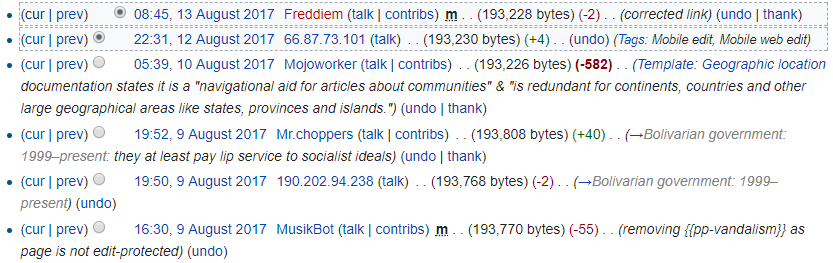
\includegraphics[scale=0.40]{images/marco_teorico/history.png}
    \captionof{figure}{Historial del artículo “Venezuela” en inglés.}
    \label{fig:marco_teorico_history}
    \bigbreak
\end{center}

Cabe destacar que cada versión o cambio provee una serie de propiedades, como: Fecha y hora de la edición, autor de la edición (si el usuario está registrado se refleja su nombre, si no, la dirección ip de su conexión), tamaño del artículo (bytes), bytes modificados, descripción de la edición, selector para identificar si el cambio es menor, y acciones para ejecutar sobre una edición (agradecer o revertir).

\begin{center}
    \bigbreak
    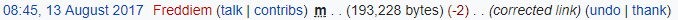
\includegraphics[scale=0.45]{images/marco_teorico/history_detail.png}
    \captionof{figure}{Propiedades de una versión del historial del artículo “Venezuela” en inglés.}
    \label{fig:marco_teorico_history_detail}
    \bigbreak
\end{center}

Adicionalmente, MediaWiki provee un API Web\footnote{\href{https://www.mediawiki.org/wiki/API:Main_page}{Página Principal del API de MediaWiki}}, esto significa que la mayoría de sus funcionalidades están expuesta en la Web y pueden ser accedidas y usadas mediante peticiones HTTP (Hypertext Transfer Protocol). De esta forma, será posible enlazar nuestro trabajo con información de Wikipedia.

\section{Visualización de datos}
La visualización de datos es un medio efectivo y eficiente para comunicar una gran cantidad de información \cite{DesignData}, en donde la comunicación está conformada por elementos visuales, contando con barras, puntos, líneas, colores, figuras, sombras, entre otras. La agrupación de estos elementos visuales se conoce como gráfica.

Como en toda comunicación, es necesario un mensajero, un mensaje y un receptor. En la visualización de datos, el papel del mensajero lo protagoniza un diseñador que codifica la información de manera visual y el receptor es el decodificador del mensaje \cite{DataVis}.

\begin{center}
    \bigbreak
    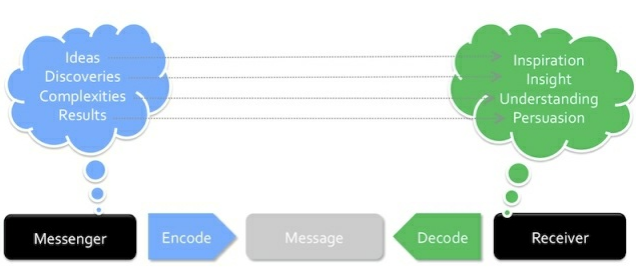
\includegraphics[scale=0.45]{images/marco_teorico/flow_vis.png}
    \captionof{figure}{Diagrama que refleja los actores y acciones de una comunicación visual}
    \label{fig:marco_teorico_flow_vis}
    \bigbreak
\end{center}

El trabajo del mensajero, que en su defecto es el diseñador, desempeña el papel más importante, debido a que tiene que transmitir una información densa usando elementos visuales, por lo tanto tiene que codificar el mensaje lo más claro y simple posible, lo que significa, que tiene que hacer uso correcto de las gráficas y lograr una buena representación de los datos.

\subsection{Enfoque explicativo y exploratorio}
En la visualización de datos se pueden tomar dos enfoques: explicativo y exploratorio.

\textbf{Explicativo:} consta de transmitir una información de manera específica, generalmente, el punto de vista del diseñador de la visualización.

\begin{center}
    \bigbreak
    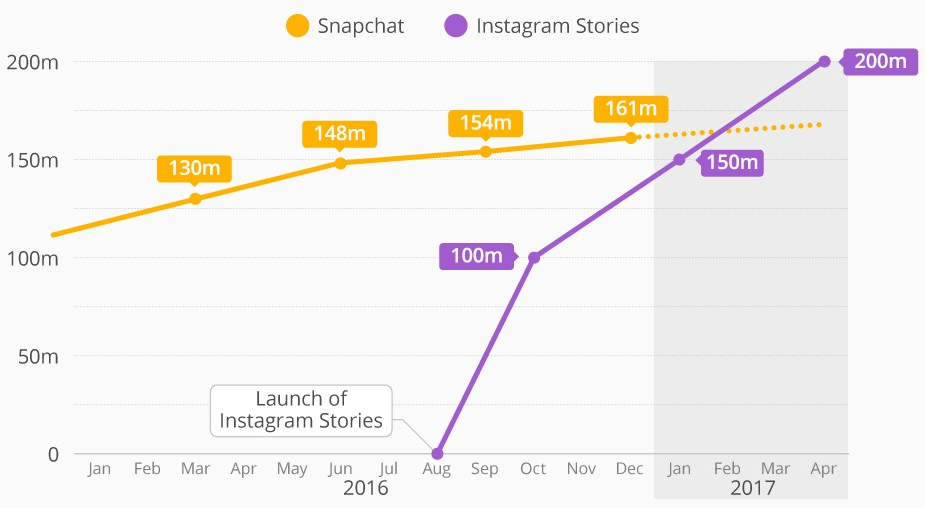
\includegraphics[scale=0.35]{images/marco_teorico/story_chart.png}
    \captionof{figure}{Usuarios activos usando “Historias” de Snapchat vs Instagram}
    \label{fig:marco_teorico_story_chart}
    \bigbreak
\end{center}

En la figura anterior \textbf{Figura \ref{fig:marco_teorico_story_chart}}, se contempla un enfoque explicativo, en donde el diseñador quiere transmitir una información concreta, que es una comparativa en el crecimiento de usuarios activos haciendo uso de la funcionalidad \textit{“Historias"}\footnote{Historias o Stories, es una funcionalidad en donde una persona puede publicar una foto durante un período de tiempo, suele ser de 24 horas.} entre la mensajería de imágenes Snapchat y la red social Instagram.

\textbf{Exploratorio:} es un enfoque en donde la gráfica está adaptada para que el receptor pueda analizar y explorar en ella, y así detectar patrones y relaciones en los datos. Este tipo de gráficas por lo general no suelen transmitir una historia como el enfoque explicativo.

\begin{center}
    \bigbreak
    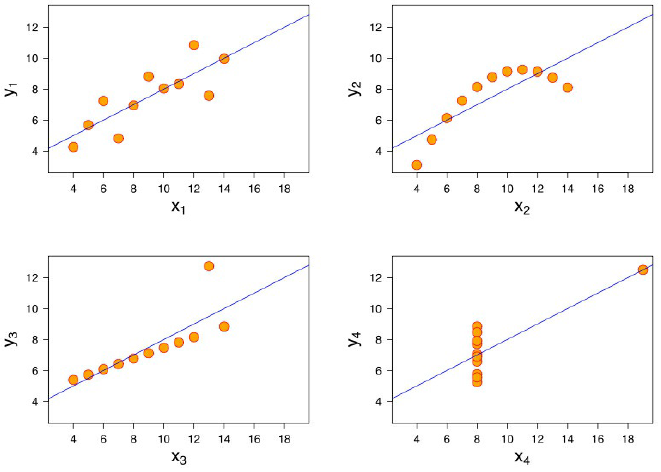
\includegraphics[scale=0.45]{images/marco_teorico/exploratory_chart.png}
    \captionof{figure}{Mediante una gráfica Scatter Plot, podemos analizar patrones y relaciones}
    \label{fig:marco_teorico_exploratory_chart}
    \bigbreak
\end{center}

En la figura anterior \textbf{Figura \ref{fig:marco_teorico_exploratory_chart}}, cada sub-gráfica representa una relación que existe entre dos (2) atributos. No existe una información concreta a transmitir, por lo tanto queda como tarea de la audiencia analizar y explorar relaciones entre atributos. Por ejemplo, el eje Y3 representa precio y eje X3 representa calidad de un producto, entonces según el comportamiento de la gráfica se interpreta que mientras más costoso es un producto mayor es su calidad.

\subsection{Preparación de los datos}
Visualizar datos no es tan sencillo como parece, en su mayoría estos datos tienen que pasar por una limpieza y procesamiento antes de ser visualizados. Si los datos a visualizar son incorrectos o están incompletos, la visualización transmitirá una información errónea. A continuación se presentarán los pasos recomendados [3] para preparar los datos:

\begin{itemize}
    \item\textbf{Adquisición:} lo principal es encontrar la fuente que nos va proveer los datos (Excel, base de datos, etc). Sin los datos es imposible continuar.
    \item\textbf{Examinación:} suelen existir datos incorrectos o incompletos, por lo tanto se debe realizar una verificación de ellos, como eliminar los duplicados, completar con otra fuente los incompletos, acomodar los datos erróneos o en el peor caso removerlos.
    \item\textbf{Estructurar los datos:} dependiendo del tipo de los datos con que contamos la visualización puede variar. Los tipos de datos se pueden dividir en: categórica nominal, categórica ordinal y cuantitativo.
    \begin{itemize}
        \item Categórica nominal: se distinguen por ser un dato que representa un valor textual. Por ejemplo: Un país, un género, etc.
        \item Categórica ordinal: es un dato nominal que puede representar un valor. Por ejemplo: Medallas Olímpicas (Oro, plata, bronce), Calor o Frío, etc.
        \item Cuantitativo: es un dato que representa un valor numérico, en donde algunos son de escala de intervalo y otros de proporción. Por ejemplo: Fechas, temperatura, precio, edad, etc.
    \end{itemize}
    \item\textbf{Limpiar:} eventualmente algunos datos pueden ser atípicos al resto, esto no dice que sean erróneos, pero pueden hacer ruido en la visualización, es buena opción eliminarlos si ese es el caso.
    \item\textbf{Transformar:} para simplificar la visualización y el análisis de la misma es posible que los datos tengan que sufrir una transformación de tipo o pre-calcular ciertas operaciones en los datos. Por ejemplo: promedio de los precios, categorizar edades (Niño: 0-12, Adolescente: 13- 19, Adulto: 20-50, Anciano: +50).
\end{itemize}

\subsection{Métodos de visualización de datos}
Toda visualización está soportada por un método de clasificación, es decir, tiene un motivo y función. A continuación algunos métodos de clasificación \cite{DataVis}:

\begin{itemize}
    \item Comparar categorías o valores
    \item Mostrar cambios en el tiempo
    \item Mostrar conexiones y relaciones
\end{itemize}

\subsection{Tipos de gráficas según método}
En esta sección se presentarán los tipos de gráficas correspondientes al método o función, mencionadas en la sección anterior, que se quiere aplicar:

\begin{itemize}
    \item\textbf{Comparar categorías:} Gráfica de puntos, Gráfica de barras, Gráfica de barras flotantes, histogramas.
    \begin{center}
        \bigbreak
        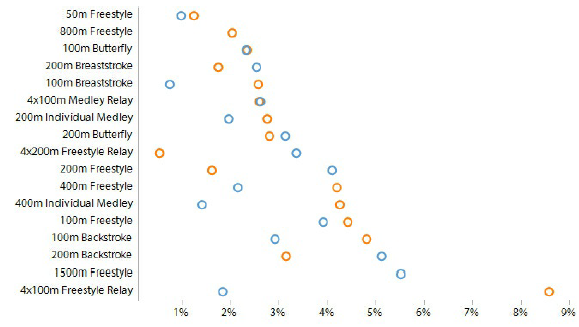
\includegraphics[scale=0.5]{images/marco_teorico/puntos_chart.png}
        \captionof{figure}{Gráfica de puntos}
        \label{fig:marco_teorico_puntos_chart}
        \bigbreak
        
        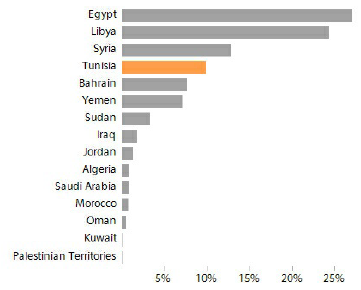
\includegraphics[scale=0.75]{images/marco_teorico/barra_chart.png}
        \captionof{figure}{Gráfica de barras}
        \label{fig:marco_teorico_barra_chart}
        \bigbreak
    
        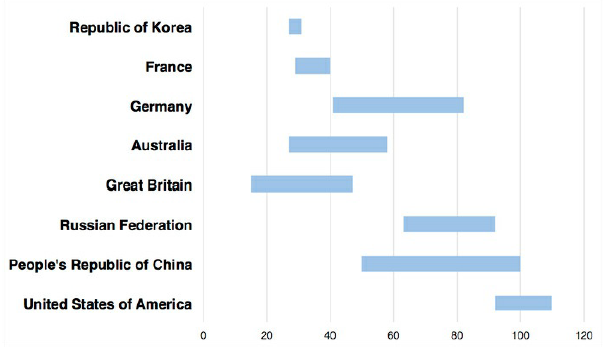
\includegraphics[scale=0.45]{images/marco_teorico/barra_flotante_chart.png}
        \captionof{figure}{Gráfica de barras flotantes}
        \label{fig:marco_teorico_barra_flotante_chart}
        \bigbreak
        
        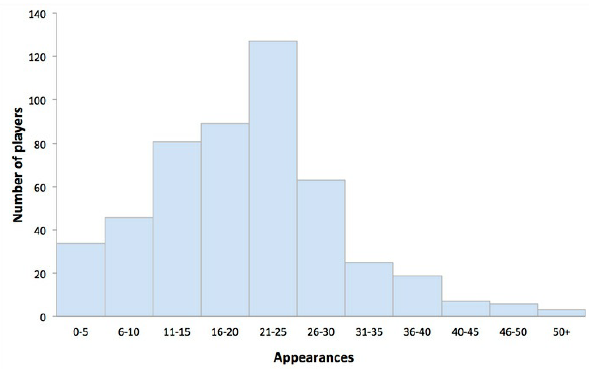
\includegraphics[scale=0.45]{images/marco_teorico/histograma_chart.png}
        \captionof{figure}{Histograma}
        \label{fig:marco_teorico_histograma_chart}
        \bigbreak
    \end{center}
    
    \item\textbf{Cambios en el tiempo:} Gráfica de línea, Gráfica de área, Gráfica de áreas apiladas.
    \begin{center}
        \bigbreak
        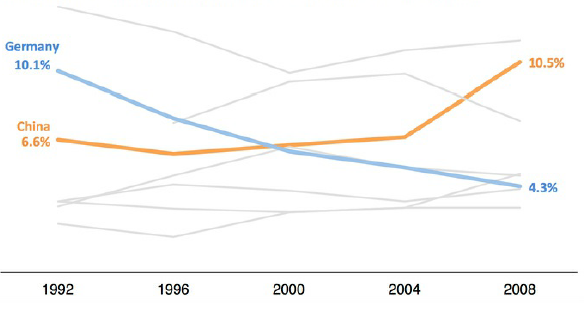
\includegraphics[scale=0.5]{images/marco_teorico/lineal_chart.png}
        \captionof{figure}{Gráfica de lineas}
        \label{fig:marco_teorico_lineal_chart}
        \bigbreak
        
        
        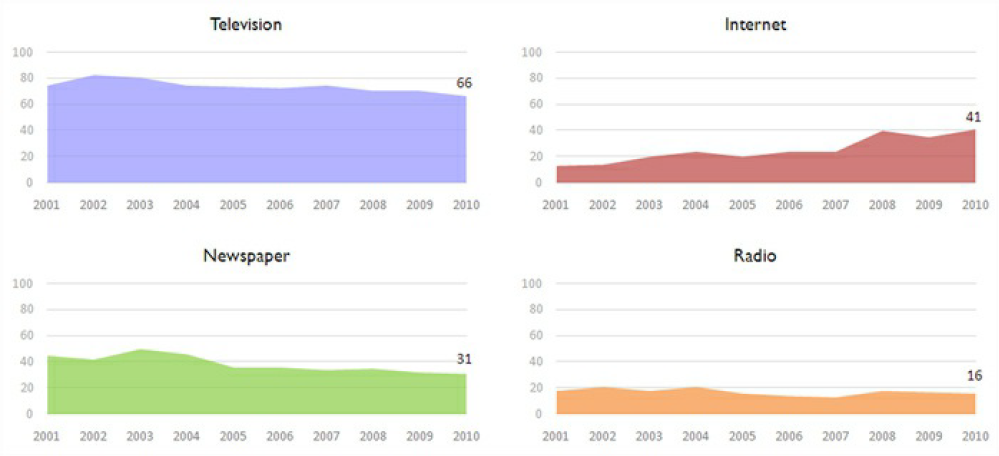
\includegraphics[scale=0.3]{images/marco_teorico/area_chart.png}
        \captionof{figure}{Gráfica de áreas}
        \label{fig:marco_teorico_area_chart}
        \bigbreak
        
        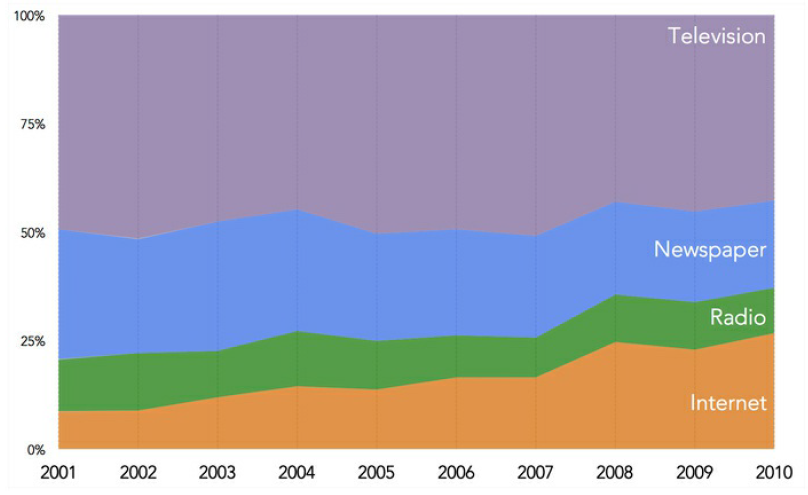
\includegraphics[scale=0.4]{images/marco_teorico/area_apilada_chart.png}
        \captionof{figure}{Gráfica de áreas apiladas}
        \label{fig:marco_teorico_area_apilada_chart}
        \bigbreak
    \end{center}
    \item\textbf{Conexiones y relaciones:} Gráfica de dispersión, Gráfica de burbujas.
    \begin{center}
        \bigbreak
        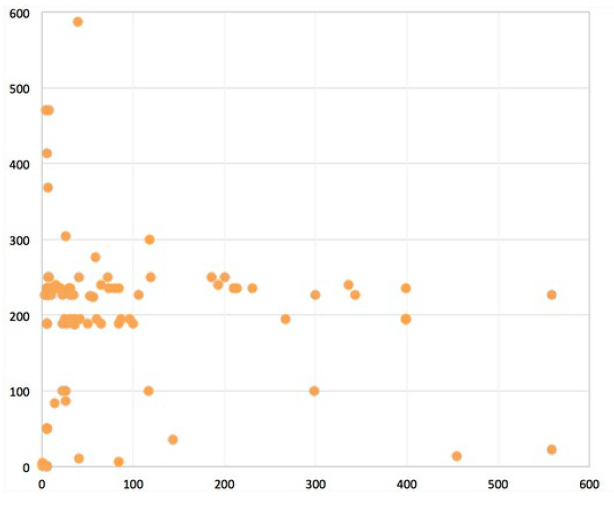
\includegraphics[scale=0.5]{images/marco_teorico/dispersion_chart.png}
        \captionof{figure}{Gráfica de dispersión}
        \label{fig:marco_teorico_dispersion_chart}
        \bigbreak
        
        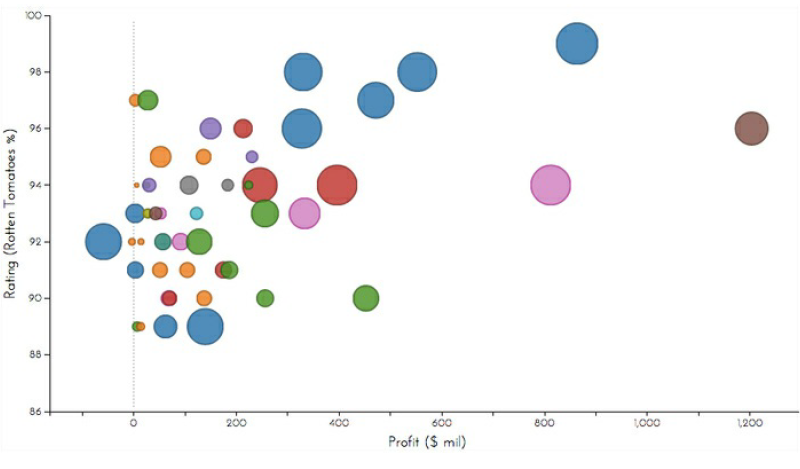
\includegraphics[scale=0.4]{images/marco_teorico/burbuja_chart.png}
        \captionof{figure}{Gráfica de burbujas}
        \label{fig:marco_teorico_burbujas_chart}
        \bigbreak
    \end{center}
\end{itemize}